\documentclass{article}
\usepackage{fullpage,amssymb,amsmath,amsthm,amsfonts,epsf}
\usepackage[12pt]{extsizes}
\usepackage{psfrag}
\usepackage{graphicx}
\usepackage{enumerate}
\usepackage{hyperref}

\newcommand{\newsec}{\section}
\newcommand{\denselist}{\itemsep 0pt\partopsep 0pt}
\newcommand{\bitem}{\begin{itemize}\denselist}
\newcommand{\eitem}{\end{itemize}}
\newcommand{\benum}{\begin{enumerate}\denselist}
\newcommand{\eenum}{\end{enumerate}}

\newcommand{\fig}[1]{\private{\begin{center}
{\Large\bf ({#1})}
\end{center}}}

\newcommand{\cpsf}[1]{{\centerline{\psfig{#1}}}}
\newcommand{\mytitle}[1]{\centerline{\LARGE\bf #1}}

\newcommand{\myw}{{\bf w}}

\newcommand{\mypar}[1]{\vspace{1ex}\noindent{\bf {#1}}}

\def\thmcolon{\hspace{-.85em} {\bf :} }

\newtheorem{THEOREM}{Theorem}[section]
\newenvironment{theorem}{\begin{THEOREM} \thmcolon }%
                        {\end{THEOREM}}
\newtheorem{LEMMA}[THEOREM]{Lemma}
\newenvironment{lemma}{\begin{LEMMA} \thmcolon }%
                      {\end{LEMMA}}
\newtheorem{COROLLARY}[THEOREM]{Corollary}
\newenvironment{corollary}{\begin{COROLLARY} \thmcolon }%
                          {\end{COROLLARY}}
\newtheorem{PROPOSITION}[THEOREM]{Proposition}
\newenvironment{proposition}{\begin{PROPOSITION} \thmcolon }%
                            {\end{PROPOSITION}}
\newtheorem{DEFINITION}[THEOREM]{Definition}
\newenvironment{definition}{\begin{DEFINITION} \thmcolon \rm}%
                            {\end{DEFINITION}}
\newtheorem{CLAIM}[THEOREM]{Claim}
\newenvironment{claim}{\begin{CLAIM} \thmcolon \rm}%
                            {\end{CLAIM}}
\newtheorem{EXAMPLE}[THEOREM]{Example}
\newenvironment{example}{\begin{EXAMPLE} \thmcolon \rm}%
                            {\end{EXAMPLE}}
\newtheorem{REMARK}[THEOREM]{Remark}
\newenvironment{remark}{\begin{REMARK} \thmcolon \rm}%
                            {\end{REMARK}}
%\newenvironment{proof}{\noindent {\bf Proof:} \hspace{.677em}}%
%                      {}

%theorem
\newcommand{\thm}{\begin{theorem}}
%lemma
\newcommand{\lem}{\begin{lemma}}
%proposition
\newcommand{\pro}{\begin{proposition}}
%definition
\newcommand{\dfn}{\begin{definition}}
%remark
\newcommand{\rem}{\begin{remark}}
%example
\newcommand{\xam}{\begin{example}}
%corollary
\newcommand{\cor}{\begin{corollary}}
%proof
\newcommand{\prf}{\noindent{\bf Proof:} }
%end theorem
\newcommand{\ethm}{\end{theorem}}
%end lemma
\newcommand{\elem}{\end{lemma}}
%end proposition
\newcommand{\epro}{\end{proposition}}
%end definition
\newcommand{\edfn}{\bbox\end{definition}}
%end remark
\newcommand{\erem}{\bbox\end{remark}}
%end example
\newcommand{\exam}{\bbox\end{example}}
%end corollary
\newcommand{\ecor}{\end{corollary}}
%end proof
\newcommand{\eprf}{\bbox\vspace{0.1in}}
%begin equation
\newcommand{\beqn}{\begin{equation}}
%end equation
\newcommand{\eeqn}{\end{equation}}

%\newcommand{\eqref}[1]{Eq.~\ref{#1}}

\newcommand{\KB}{\mbox{\it KB\/}}
\newcommand{\infers}{\vdash}
\newcommand{\sat}{\models}
\newcommand{\bbox}{\vrule height7pt width4pt depth1pt}

\newcommand{\act}[1]{\stackrel{{#1}}{\rightarrow}}
\newcommand{\at}[1]{^{(#1)}}

\newcommand{\argmax}{{\rm argmax}}

\newcommand{\rimp}{\Rightarrow}
\newcommand{\dimp}{\Leftrightarrow}

\newcommand{\bX}{\mbox{\boldmath $X$}}
\newcommand{\bY}{\mbox{\boldmath $Y$}}
\newcommand{\bZ}{\mbox{\boldmath $Z$}}
\newcommand{\bU}{\mbox{\boldmath $U$}}
\newcommand{\bE}{\mbox{\boldmath $E$}}
\newcommand{\bx}{\mbox{\boldmath $x$}}
\newcommand{\be}{\mbox{\boldmath $e$}}
\newcommand{\by}{\mbox{\boldmath $y$}}
\newcommand{\bz}{\mbox{\boldmath $z$}}
\newcommand{\bu}{\mbox{\boldmath $u$}}
\newcommand{\bd}{\mbox{\boldmath $d$}}
\newcommand{\smbx}{\mbox{\boldmath $\scriptstyle x$}}
\newcommand{\smbd}{\mbox{\boldmath $\scriptstyle d$}}
\newcommand{\smby}{\mbox{\boldmath $\scriptstyle y$}}
\newcommand{\smbe}{\mbox{\boldmath $\scriptstyle e$}}


\newcommand{\word}[1]{\mbox{\it #1\/}}
\newcommand{\Action}{\word{Action}}
\newcommand{\Proposition}{\word{Proposition}}
\newcommand{\true}{\word{true}}
\newcommand{\false}{\word{false}}
\newcommand{\Pre}{\word{Pre}}
\newcommand{\Add}{\word{Add}}
\newcommand{\Del}{\word{Del}}
\newcommand{\Result}{\word{Result}}
\newcommand{\Regress}{\word{Regress}}
\newcommand{\Maintain}{\word{Maintain}}

\newcommand{\bor}{\bigvee}
\newcommand{\invert}[1]{{#1}^{-1}}

\newcommand{\commentout}[1]{}

\newcommand{\bmu}{\mbox{\boldmath $\mu$}}
\newcommand{\btheta}{\mbox{\boldmath $\theta$}}
\newcommand{\IR}{\mbox{$I\!\!R$}}

\newcommand{\tval}[1]{{#1}^{1}}
\newcommand{\fval}[1]{{#1}^{0}}

\newcommand{\tr}{{\rm tr}}
\newcommand{\vecy}{{\vec{y}}}
\renewcommand{\Re}{{\mathbb R}}

\def\twofigbox#1#2{%
\noindent\begin{minipage}{\textwidth}%
\epsfxsize=0.35\maxfigwidth
\noindent \epsffile{#1}\hfill
\epsfxsize=0.35\maxfigwidth
\epsffile{#2}\\
\makebox[0.35\textwidth]{(a)}\hfill\makebox[0.35\textwidth]{(b)}%
\end{minipage}}

\def\twofigboxcd#1#2{%
\noindent\begin{minipage}{\textwidth}%
\epsfxsize=0.35\maxfigwidth
\noindent \epsffile{#1}\hfill
\epsfxsize=0.35\maxfigwidth
\epsffile{#2}\\
\makebox[0.35\textwidth]{(c)}\hfill\makebox[0.35\textwidth]{(d)}%
\end{minipage}}

\def\twofigboxnolabel#1#2{%
\begin{minipage}{\textwidth}%
\epsfxsize=0.35\maxfigwidth
\noindent \epsffile{#1}\hfill
\epsfxsize=0.35\maxfigwidth
\epsffile{#2}\\
%\makebox[0.48\textwidth]{(a)}\hfill\makebox[0.48\textwidth]{(b)}%
\end{minipage}
}

\def\twofigboxnolabelFive#1#2{%
\begin{minipage}{\textwidth}%
\hbox to 0.5in{}\epsfxsize=0.35\maxfigwidth
\noindent \epsffile{#1}\hfill
\epsfxsize=0.35\maxfigwidth
\epsffile{#2}\hbox to 0.5in{}\\
%\makebox[0.48\textwidth]{(a)}\hfill\makebox[0.48\textwidth]{(b)}%
\end{minipage}
}

\def\threefigbox#1#2#3{%
\noindent\begin{minipage}{\textwidth}%
\epsfxsize=0.33\maxfigwidth
\noindent \epsffile{#1}\hfill
\epsfxsize=0.33\maxfigwidth
\noindent \epsffile{#2}\hfill 
\epsfxsize=0.33\maxfigwidth
\epsffile{#3}\\
\makebox[0.31\textwidth]{{\scriptsize (a)}}\hfill%
\makebox[0.31\textwidth]{{\scriptsize (b)}}\hfill
\makebox[0.31\textwidth]{{\scriptsize (c)}}%
\smallskip
\end{minipage}}

\def\threefigboxnolabel#1#2#3{%
\noindent\begin{minipage}{\textwidth}%
\epsfxsize=0.33\maxfigwidth
\noindent \epsffile{#1}\hfill
\epsfxsize=0.33\maxfigwidth
\noindent \epsffile{#2}\hfill 
\epsfxsize=0.33\maxfigwidth
\epsffile{#3}\\
%\makebox[0.31\textwidth]{{\scriptsize (a)}}\hfill%
%\makebox[0.31\textwidth]{{\scriptsize (b)}}\hfill
%\makebox[0.31\textwidth]{{\scriptsize (c)}}%
%\smallskip
\end{minipage}}

\newlength{\maxfigwidth}
\setlength{\maxfigwidth}{\textwidth}
%\def\captionsize {\footnotesize}
\def\captionsize {}

\newcommand{\xsi}{{x^{(i)}}}
\newcommand{\xsd}{{x^{(d)}}}
\newcommand{\xsj}{{x^{(j)}}}
\newcommand{\ysi}{{y^{(i)}}}
\newcommand{\ysj}{{y^{(j)}}}
\newcommand{\gsi}{{\gamma^{(i)}}}
\newcommand{\wsi}{{w^{(i)}}}
\newcommand{\esi}{{\epsilon^{(i)}}}

\newcommand{\calM}{{\cal M}}
\newcommand{\calH}{{\cal H}}
\newcommand{\calN}{{\cal N}}
\newcommand{\calX}{{\cal X}}
\newcommand{\calY}{{\cal Y}}
\newcommand{\calL}{{\cal L}}
\newcommand{\calP}{{\cal P}}
\newcommand{\calD}{{\cal D}}
\newcommand{\calF}{{\cal F}}

\newcommand{\ytil}{{\tilde{y}}}

\newcommand{\Ber}{{\rm Bernoulli}}
\newcommand{\MI}{{\rm MI}}
\newcommand{\E}{{\rm E}}

\newcommand{\pstar}{{p^{\ast}}}
\newcommand{\bstar}{{b^{\ast}}}
\newcommand{\dstar}{{d^{\ast}}}
\newcommand{\wstar}{{w^{\ast}}}
\newcommand{\alphastar}{\alpha^{\ast}}
\newcommand{\alphastari}{{\alpha_i^{\ast}}}
\newcommand{\betastar}{{\beta^{\ast}}}
\newcommand{\tol}{{\textit tol}}
\newcommand{\phihat}{\hat\phi}
\newcommand{\ehat}{\hat\varepsilon}
\newcommand{\hhat}{\hat{h}}
\newcommand{\hstar}{h^\ast}
\newcommand{\VC}{{\rm VC}}

\newcommand{\Strain}{S_{\rm train}}
\newcommand{\Scv}{{S_{\rm cv}}}

\newcommand{\hwb}{{h_{w,b}}}


\newcommand{\represent}{\phi}

\begin{document}
\title{XCS229i Supplemental Lecture Notes}
\author{Andrew Ng}
%\date{Lectures from 1/7/03 to 1/16/03}
\date{}
\maketitle

\section{Boosting}

We have seen so far how to solve classification (and other) problems when we
have a data representation already chosen. We now talk about a procedure,
known as \emph{boosting}, which was originally discovered by Rob Schapire,
and further developed by Schapire and Yoav Freund, that automatically
chooses feature representations. We take an optimization-based perspective,
which is somewhat different from the original interpretation and
justification of Freund and Schapire, but which lends itself to our approach
of (1) choose a representation, (2) choose a loss, and (3) minimize the
loss.

Before formulating the problem, we give a little intuition for what we are
going to do. Roughly, the idea of boosting is to take a \emph{weak learning}
algorithm---any learning algorithm that gives a classifier that is slightly
better than random---and transforms it into a \emph{strong} classifier,
which does much much better than random. To build a bit of intuition for
what this means, consider a hypothetical digit recognition experiment, where
we wish to distinguish $0$s from $1$s, and we receive images we must
classify. Then a natural weak learner might be to take the middle pixel of
the image, and if it is colored, call the image a $1$, and if it is blank,
call the image a $0$. This classifier may be far from perfect, but it is
likely better than random. Boosting procedures proceed by taking a
collection of such weak classifiers, and then reweighting their
contributions to form a classifier with much better accuracy than any
individual classifier.

With that in mind, let us formulate the problem. Our interpretation of
boosting is as a coordinate descent method in an infinite dimensional space,
which---while it sounds complex---is not so bad as it seems. First,
we assume we have raw input examples $x \in \R^n$ with labels $y \in \{-1,
1\}$, as is usual in binary classification. We also assume we have an
infinite collection of \emph{feature} functions $\represent_j : \R^n \to \{-1, 1\}$
and an infinite vector $\theta = [\theta_1 ~ \theta_2 ~ \cdots ]^T$, but
which we assume always has only a finite number of non-zero entries. For our
classifier we use
\begin{equation*}
  h_\theta(x) = \sign\bigg(\sum_{j = 1}^\infty \theta_j \represent_j(x) \bigg).
\end{equation*}
We will abuse notation, and define $\theta^T \represent(x) = \sum_{j = 1}^\infty
\theta_j \represent_j(x)$.

\newcommand{\indic}[1]{1\left\{{#1}\right\}}
\newcommand{\argmin}{\mathop{\rm arg\hspace{.1em}min}}

In boosting, one usually calls the features $\represent_j$ \emph{weak hypotheses}.
Given a training set $(x^{(1)}, y^{(1)}), \ldots, (x^{(m)}, y^{(m)})$,
we call a vector $p = (p^{(1)}, \ldots, p^{(m)})$ a distribution on the
examples if $p^{(i)} \ge 0$ for all $i$ and
\begin{equation*}
  \sum_{i = 1}^m p^{(i)} = 1.
\end{equation*}
Then we say that there is a \emph{weak learner with margin $\gamma > 0$} if
for any distribution $p$ on the $m$ training examples there exists
one weak hypothesis $\represent_j$ such that
\begin{equation}
  \label{eqn:weak-learnability}
  \sum_{i = 1}^m p^{(i)} \indic{y^{(i)} \neq \represent_j(\xsi)}
  \le \half - \gamma.
\end{equation}
That is, we assume that there is \emph{some} classifier that does slightly
better than random guessing on the dataset. The existence of a weak learning
algorithm is an assumption, but the surprising thing is that we can
transform any weak learning algorithm into one with perfect accuracy.

In more generality, we assume we have access to a \emph{weak learner},
which is an algorithm that takes as input a distribution (weights)
$p$ on the training examples and returns a classifier doing slightly
better than random.
\begin{figure}[h!]
  \begin{center}
    \algbox{
      \begin{enumerate}[(i)]
      \item \textbf{Input:} A distribution $p^{(1)}, \ldots, p^{(m)}$ and
        training set $\{(\xsi, \ysi)\}_{i=1}^m$
        with $\sum_{i = 1}^m p^{(i)} = 1$ and $p^{(i)} \ge 0$
      \item \textbf{Return:} A weak classifier $\represent_j : \R^n \to \{-1, 1\}$ such
        that
        \begin{equation*}
          \sum_{i = 1}^m p^{(i)}
          \indic{\ysi \neq \represent_j(\xsi)} \le \half - \gamma.
        \end{equation*}
      \end{enumerate}
    }
    \caption{\label{fig:weak-learning} Weak learning algorithm}
  \end{center}
\end{figure}
We will show how, given access to a weak learning algorithm, boosting can
return a classifier with perfect accuracy on the training data.
(Admittedly, we would like the classifier to generalize well to unseen data,
but for now, we ignore this issue.)

\subsection{The boosting algorithm}

Roughly, boosting begins by assigning each training example equal weight in
the dataset. It then receives a weak-hypothesis that does well according to
the current weights on training examples, which it incorporates into its
current classification model. It then reweights the training examples so
that examples on which it makes mistakes receive higher weight---so that the
weak learning algorithm focuses on a classifier doing well on those
examples---while examples with no mistakes receive lower weight. This
repeated reweighting of the training data coupled with a weak learner doing
well on examples for which the classifier currently does poorly yields
classifiers with good performance.

The boosting algorithm specifically performs \emph{coordinate descent}
on the exponential loss for classification problems, where the
objective is
\begin{equation*}
  J(\theta) = \frac{1}{m} \sum_{i = 1}^m \exp(-\ysi \theta^T \represent(\xsi)).
\end{equation*}
We first show how to compute the exact form of the coordinate descent
update for the risk $J(\theta)$. Coordinate descent iterates as follows:
\begin{enumerate}[(i)]
\item Choose a coordinate $j \in \N$
\item Update $\theta_j$ to
  \begin{equation*}
    \theta_j = \argmin_{\theta_j} J(\theta)
  \end{equation*}
  while leaving $\theta_k$ identical for all $k \neq j$.
\end{enumerate}
We iterate the above procedure until convergence.

In the case of boosting, the coordinate updates are not too challenging to
derive because of the analytic convenience of the $\exp$ function.
We now show how to derive the update. Suppose we wish to update
coordinate $j$. Define
\begin{equation*}
  w^{(i)} = \exp\left(-\ysi \sum_{k \neq j} \theta_k \represent_k(\xsi)\right)
\end{equation*}
to be a weight, and let $\alpha = \theta_j$. We can then express
\begin{equation*}
  J(\theta) = \frac{1}{m} \sum_{i = 1}^m w^{(i)} \exp(-\ysi \represent_j(\xsi) \alpha)
\end{equation*}
Now, define
\begin{equation*}
  W^+ \defeq \sum_{i : \ysi \represent_j(\xsi) = 1} w^{(i)}
  ~~ \mbox{and} ~~
  W^- \defeq \sum_{i : \ysi \represent_j(\xsi) = -1} w^{(i)}
\end{equation*}
to be the sums of the weights of examples that $\represent_j$ classifies correctly
and incorrectly, respectively. Then finding $\theta_j$ is the same as choosing
\begin{equation*}
  \alpha = \argmin_{\alpha} \left\{ W^+ e^{-\alpha}
  + W^- e^\alpha \right\}
  = \half \log \frac{W^+}{W^-}.
\end{equation*}
To see the final equality, take derivatives and set the resulting
equation to zero, so we have $-W^+ e^{-\alpha} +
W^- e^\alpha = 0$.  That is, $W^- e^{2\alpha} = W^+$, or $\alpha = \half \log
\frac{W^+}{W^-}$.


What remains is to choose the particular coordinate to perform coordinate
descent on. We assume we have access to a weak-learning algorithm as in
Figure~\ref{fig:weak-learning}, which at iteration $t$ takes as input a
distribution $p$ on the training set and returns a weak hypothesis $\represent_t$
satisfying the margin condition~\eqref{eqn:weak-learnability}.  We present
the full boosting algorithm in Figure~\ref{fig:boosting}. It proceeds in
iterations $t =1, 2, 3, \ldots$. We represent the set of hypotheses returned
by the weak learning algorithm at time $t$ by $\{\represent_1, \ldots, \represent_t\}$.
\begin{figure}
  \begin{center}
    \algbox{
      For each iteration $t = 1, 2, \ldots$:
      \begin{enumerate}[(i)]
      \item Define weights
        \begin{equation*}
          w^{(i)} = \exp\bigg(-\ysi \sum_{\tau = 1}^{t-1} \theta_\tau
          \represent_\tau(\xsi)\bigg)
        \end{equation*}
        and distribution $p^{(i)} = w^{(i)} / \sum_{j = 1}^m w^{(j)}$
      \item Construct a weak hypothesis $\represent_t : \R^n \to \{-1, 1\}$ from the
        distribution $p = (p^{(1)}, \ldots, p^{(m)})$ on the training set
      \item Compute $W_t^+ = \sum_{i : \ysi \represent_t(\xsi) = 1} w^{(i)}$
        and $W_t^- = \sum_{i : \ysi \represent_t(\xsi) = -1} w^{(i)}$ and set
        \begin{equation*}
          \theta_t = \half \log \frac{W_t^+}{W_t^-}.
        \end{equation*}
      \end{enumerate}
    }
    \caption{\label{fig:boosting} Boosting algorithm}
  \end{center}
\end{figure}

\section{The convergence of Boosting}

\renewenvironment{proof}{\noindent{\bf Proof}\hspace*{1em}}{\qed\medskip\\}

We now argue that the boosting procedure achieves 0 training error,
and we also provide a rate of convergence to zero.
To do so, we present a lemma that guarantees progress is made.
\begin{lemma}
  \label{lemma:boosting-progress}
  Let
  \begin{equation*}
    J(\theta^{(t)})
    = \frac{1}{m} \sum_{i = 1}^m \exp\bigg(-\ysi \sum_{\tau = 1}^t
    \theta_\tau \represent_\tau(\xsi)\bigg).
  \end{equation*}
  Then
  \begin{equation*}
    J(\theta^{(t)})
    \le \sqrt{1 - 4 \gamma^2} J(\theta^{(t - 1)}).
  \end{equation*}
\end{lemma}
\noindent
As the proof of the lemma is somewhat involved and not the central focus of
these notes---though it is important to know one's algorithm will
converge!---we defer the proof to
Appendix~\ref{sec:proof-boosting-progress}.
Let us describe how it guarantees convergence of the
boosting procedure to a classifier with zero training error.

%% TODO: Get the sign thing fixed up with sgn.

We initialize the procedure at $\theta^{(0)} = \vec{0}$,
so that the initial empirical risk $J(\theta^{(0)}) = 1$. Now, we note
that for any $\theta$, the misclassification error satisfies
\begin{equation*}
  \indic{\sign(\theta^T \represent(x)) \neq y}
  = \indic{y \theta^T \represent(x) \le 0}
  \le \exp\left(-y \theta^T \represent(x)\right)
\end{equation*}
because $e^z \ge 1$ for all $z \ge 0$. Thus, we have that the
misclassification error rate has upper bound
\begin{equation*}
  \frac{1}{m} \sum_{i = 1}^m \indic{\sign(\theta^T \represent(\xsi)) \neq \ysi}
  \le J(\theta),
\end{equation*}
and so if $J(\theta) < \frac{1}{m}$ then the vector $\theta$ makes \emph{no}
mistakes on the training data.
After $t$ iterations of boosting, we find that the empirical risk satisfies
\begin{equation*}
  J(\theta^{(t)})
  \le (1 - 4 \gamma^2)^\frac{t}{2} J(\theta^{(0)})
  = (1 - 4 \gamma^2)^\frac{t}{2}.
\end{equation*}
To find how many iterations are required to guarantee
$J(\theta^{(t)}) < \frac{1}{m}$, we take logarithms to
find that $J(\theta^{(t)}) < 1/m$ if
\begin{equation*}
  \frac{t}{2} \log(1 - 4 \gamma^2) < \log \frac{1}{m},
  ~~ \mbox{or} ~~
  t > \frac{2 \log m}{-\log(1 - 4 \gamma^2)}.
\end{equation*}
Using a first order Taylor expansion, that is, that
$\log(1 - 4 \gamma^2) \le -4\gamma^2$, we see that if the number
of rounds of boosting---the number of weak classifiers we use---satisfies
\begin{equation*}
  t > \frac{\log m}{2 \gamma^2}
  \ge \frac{2 \log m}{-\log(1 - 4 \gamma^2)},
\end{equation*}
then $J(\theta^{(t)}) < \frac{1}{m}$.

\section{Implementing weak-learners}

One of the major advantages of boosting algorithms is that they
automatically generate features from raw data for us. Moreover, because the
weak hypotheses always return values in $\{-1, 1\}$, there is no need to
normalize features to have similar scales when using learning algorithms,
which in practice can make a large difference.  Additionally, and while this
is not theoretically well-understood, many types of weak-learning procedures
introduce non-linearities intelligently into our classifiers, which can
yield much more expressive models than the simpler linear models of the form
$\theta^T x$ that we have seen so far.

\subsection{Decision stumps}

There are a number of strategies for weak learners, and here
we focus on one, known as \emph{decision stumps}. For concreteness in this
description, let us suppose that the input variables $x \in \R^n$
are real-valued. A decision stump is a function $f$, which is parameterized
by a threshold $s$ and index $j \in \{1, 2, \ldots, n\}$, and returns
\begin{equation}
  \label{eqn:stumpy}
  \represent_{j,s}(x) = \sign(x_j - s)
  = \begin{cases} 1 & \mbox{if~} x_j \ge s \\ -1 & \mbox{otherwise}.
  \end{cases}
\end{equation}
These classifiers are simple enough that we can fit them efficiently
even to a weighted dataset, as we now describe.

\newcommand{\what}[1]{\widehat{#1}}

Indeed, a decision stump weak learner proceeds as follows. We begin
with a distribution---set of weights $p^{(1)}, \ldots, p^{(m)}$ summing
to $1$---on the training set, and we wish to choose a decision
stump of the form~\eqref{eqn:stumpy} to minimize the error on the
training set. That is, we wish to find a threshold
$s \in \R$ and index $j$ such that
\begin{equation}
  \label{eqn:stump-error}
  \what{\rm Err}(\represent_{j,s}, p)
  = \sum_{i = 1}^m p^{(i)} \indic{\represent_{j,s}(\xsi) \neq \ysi}
  = \sum_{i = 1}^m p^{(i)} \indic{\ysi (x_j^{(i)} - s) \le 0}
\end{equation}
is minimized. Naively, this could be an inefficient calculation, but
a more intelligent procedure allows us to solve this problem in roughly
$O(nm \log m)$ time. For each feature $j = 1, 2, \ldots, n$, we sort
the raw input features so that
\begin{equation*}
  x_j^{(i_1)} \ge x_j^{(i_2)} \ge \cdots \ge x_j^{(i_m)}.
\end{equation*}
As the only values $s$ for which the error of the decision stump
can change are the values $x_j^{(i)}$, a bit of clever book-keeping
allows us to compute
\begin{equation*}
  \sum_{i = 1}^m p^{(i)} \indic{y^{(i)}(x_j^{(i)} - s) \le 0}
  = \sum_{k = 1}^m p^{(i_k)} \indic{y^{(i_k)} (x_j^{(i_k)} - s) \le 0}
\end{equation*}
efficiently by incrementally modifying the sum in sorted order, which takes
time $O(m)$ after we have already sorted the values $x_j^{(i)}$.  (We do not
describe the algorithm in detail here, leaving that to the interested
reader.) Thus, performing this calculation for each of the $n$ input features
takes total time $O(nm \log m)$, and we may choose the index $j$ and
threshold $s$ that give the best decision stump for the
error~\eqref{eqn:stump-error}.

One \emph{very} important issue to note is that by flipping the sign of the
thresholded decision stump $\represent_{j,s}$, we achieve error $1 - \what{\rm
  Err}(\represent_{j, s}, p)$, that is, the error of
\begin{equation*}
  \what{\rm Err}(-\represent_{j, s}, p) =
  1 - \what{\rm Err}(\represent_{j, s}, p).
\end{equation*}
(You should convince yourself that this is true.)
Thus, it is important to also track the smallest value of $1 - \what{\rm
  Err}(\represent_{j,s}, p)$ over all thresholds, because this may be smaller than
$\what{\rm Err}(\represent_{j,s}, p)$, which gives a better weak learner.
Using this procedure for our weak learner (Fig.~\ref{fig:weak-learning})
gives the basic, but extremely useful, boosting classifier.

\subsection{Example}

\begin{figure}[ht]
  \begin{center}
    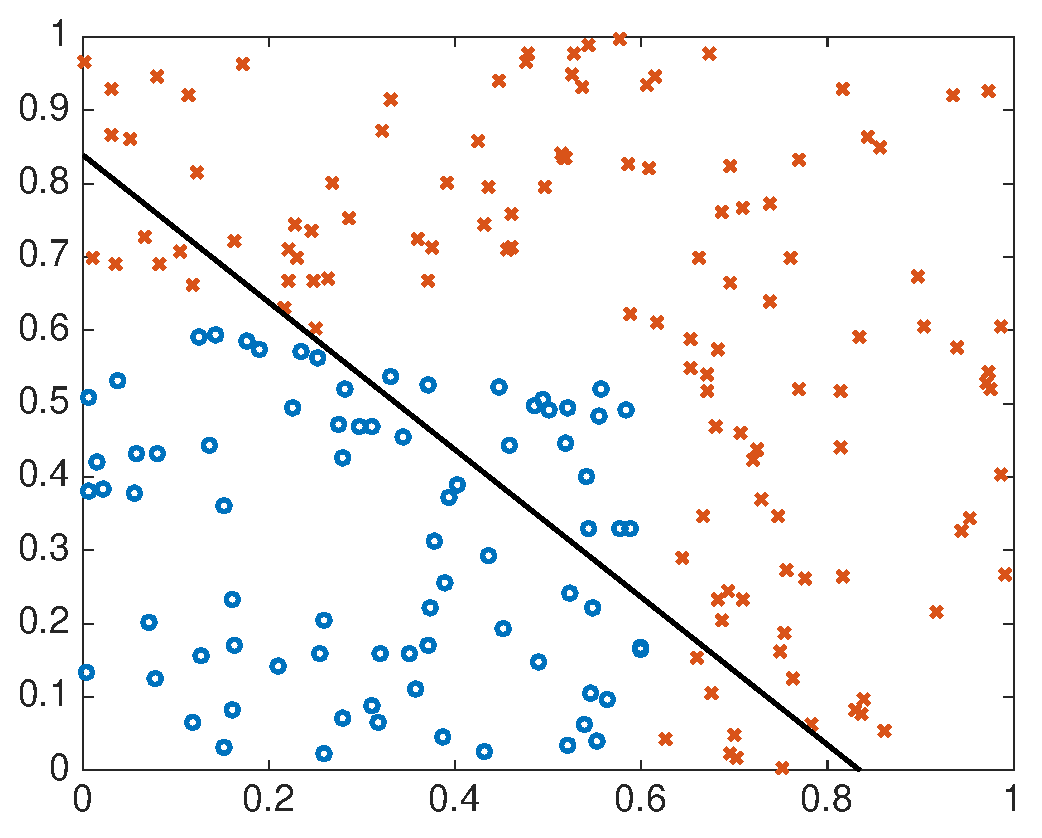
\includegraphics[width=.6\columnwidth]{logistic_plot.eps}
    \caption{\label{fig:logreg} Best logistic regression classifier
      using the raw features $x \in \R^2$ (and a bias term $x_0 = 1$)
      for the example considered here.}
  \end{center}
\end{figure}


We now give an example showing the behavior of boosting on a simple dataset.
In particular, we consider a problem with data points $x \in \R^2$, where
the optimal classifier is
\begin{equation}
  \label{eqn:simple-nonlinear}
  y = \begin{cases} 1 & \mbox{if~} x_1 < .6 ~\mbox{and}~ x_2 < .6 \\
    -1 & \mbox{otherwise}.
  \end{cases}
\end{equation}
This is a simple non-linear decision rule, but it is impossible for standard
linear classifiers, such as logistic regression, to learn.  In
Figure~\ref{fig:logreg}, we show the best decision line that logistic
regression learns, where positive examples are circles and negative examples
are x's. It is clear that logistic regression is not fitting the data
particularly well.

With boosted decision stumps, however, we can achieve a much better fit for
the simple nonlinear classification problem~\eqref{eqn:simple-nonlinear}.
Figure~\ref{fig:boosty} shows the boosted classifiers we have learned after
different numbers of iterations of boosting, using a training set of size $m
= 150$. From the figure, we see that the first decision stump is to
threshold the feature $x_1$ at the value $s \approx .23$, that is,
$\represent(x) = \sign(x_1 - s)$ for $s \approx .23$.
\begin{figure}
  \begin{center}
    \begin{tabular}{cc}
      \psfrag{Iterations = 2}{2 Iterations}
      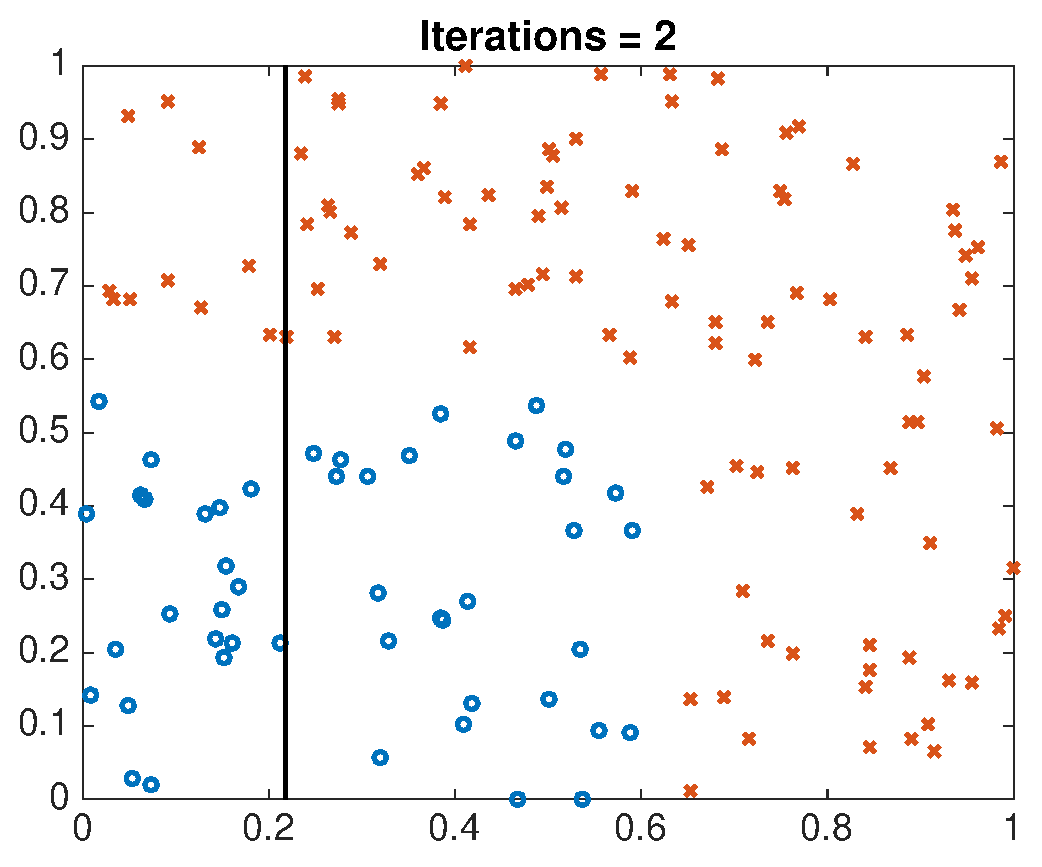
\includegraphics[width=.5\columnwidth]{boost_plot_2} &
      \psfrag{Iterations = 4}{4 Iterations}
      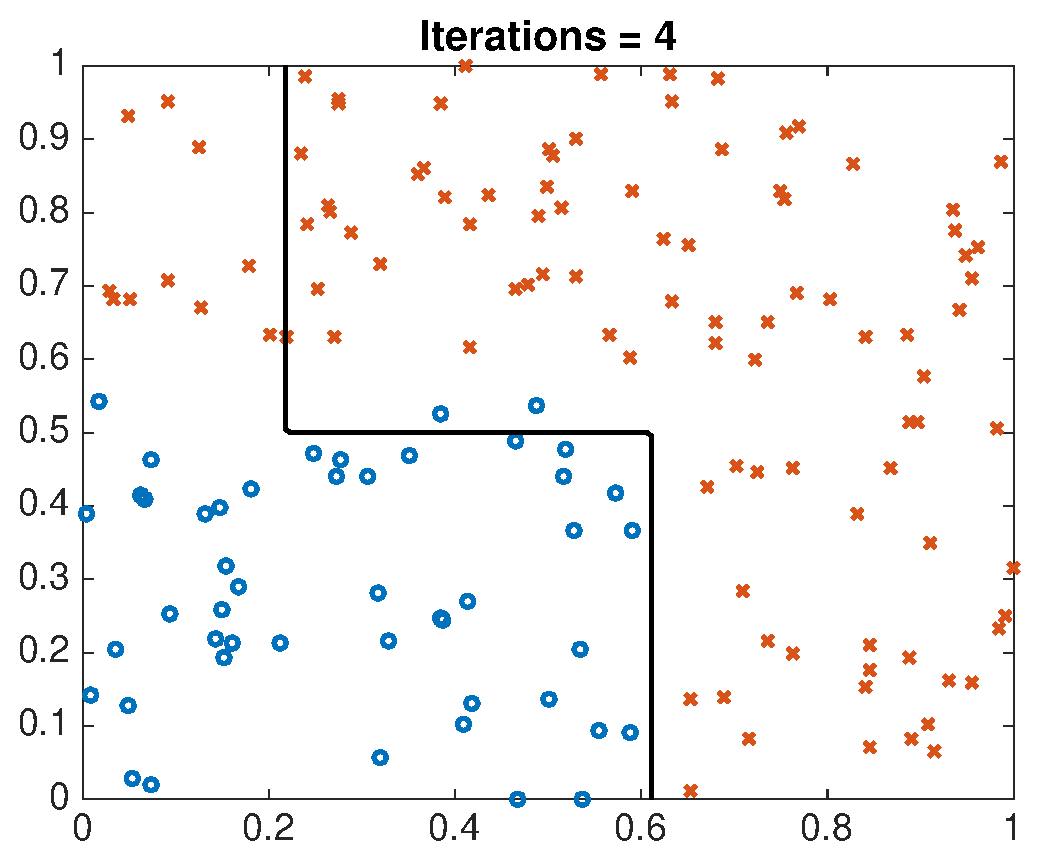
\includegraphics[width=.5\columnwidth]{boost_plot_4} \\
      \psfrag{Iterations = 5}{5 Iterations}
      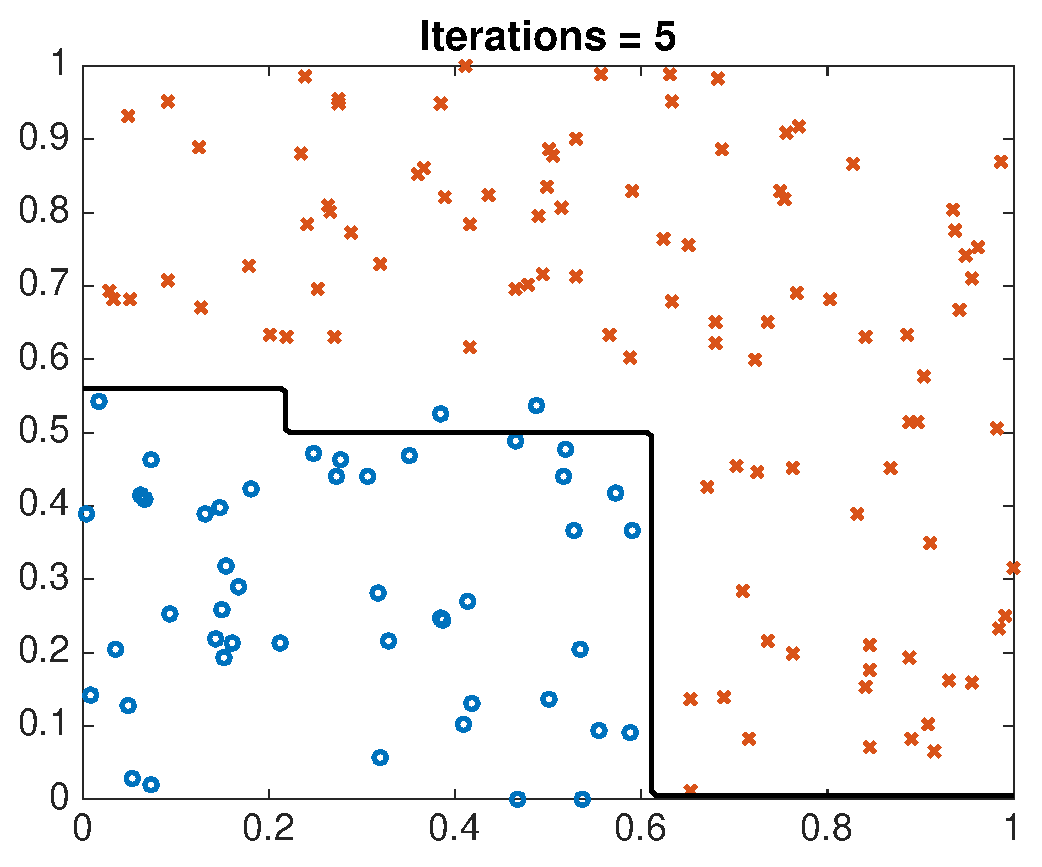
\includegraphics[width=.5\columnwidth]{boost_plot_5} &
      \psfrag{Iterations = 10}{10 Iterations}
      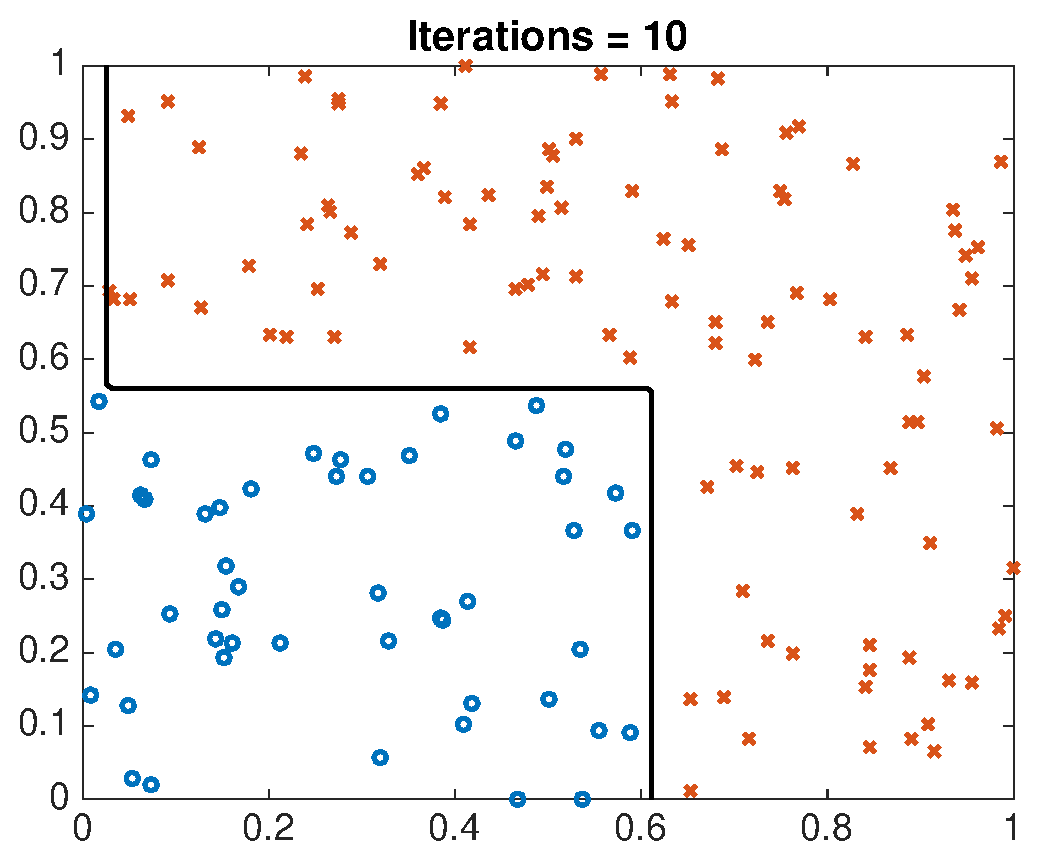
\includegraphics[width=.5\columnwidth]{boost_plot_10}
    \end{tabular}
    \caption{\label{fig:boosty} Boosted decision stumps after
      $t = 2, 4, 5$, and $10$ iterations of boosting, respectively.}
  \end{center}
\end{figure}

\subsection{Other strategies}

There are a huge number of variations on the basic boosted decision stumps
idea. First, we do not require that the input features $x_j$ be real-valued.
Some of them may be categorical, meaning that $x_j \in \{1, 2, \ldots, k\}$
for some $k$, in which case natural decision stumps are of the form
\begin{equation*}
  \represent_j(x) = \begin{cases} 1 & \mbox{if~} x_j = l \\
    -1 & \mbox{otherwise}, \end{cases}
\end{equation*}
as well as variants setting $\represent_j(x) = 1$ if $x_j \in C$
for some set $C \subset \{1, \ldots, k\}$ of categories.

Another natural variation is the \emph{boosted decision tree}, in which
instead of a single level decision for the weak learners, we consider
conjunctions of features or trees of decisions. Google can help you find
examples and information on these types of problems.

\appendix
\section{Appendices}

\subsection{Proof of Lemma~\ref{lemma:boosting-progress}}
\label{sec:proof-boosting-progress}

We now return to prove the progress lemma. We prove this result by directly
showing the relationship of the weights at time $t$ to those at time
$t-1$. In particular, we note by inspection that
\begin{equation*}
  J(\theta^{(t)})
  = \frac{1}{m} \min_{\alpha} \{ W_t^+ e^{-\alpha} + W_t^- e^\alpha\}
  = \frac{2}{m} \sqrt{ W_t^+ W_t^-}
\end{equation*}
while
\begin{equation*}
  J(\theta^{(t - 1)})
  = \frac{1}{m} \sum_{i = 1}^m \exp\bigg(-\ysi \sum_{\tau = 1}^{t-1}
  \theta_\tau \represent_\tau(\xsi)\bigg)
  = \frac{1}{m} \bigg(W_t^+ + W_t^-\bigg).
\end{equation*}

We know by the weak-learning assumption that
\begin{equation*}
  \sum_{i = 1}^m p^{(i)} \indic{y^{(i)} \neq \represent_t(\xsi)} \le
  \half - \gamma,
  ~~ \mbox{or} ~~
  \frac{1}{W_t^+ + W_t^-}
  \underbrace{\sum_{i : \ysi \represent_t(\xsi) = -1}
    w^{(i)}}_{= W_t^-} \le \half - \gamma.
\end{equation*}
Rewriting this expression by noting that the sum on the right is $W_t^-$, we have
\begin{equation*}
  W_t^- \le \left(\half - \gamma\right) (W_t^+ + W_t^-),
  ~~ \mbox{or} ~~
  W_t^+ \ge \frac{1 + 2 \gamma}{1 - 2 \gamma} W_t^-.
\end{equation*}
By substituting $\alpha = \half \log \frac{1 + 2 \gamma}{1 - 2 \gamma}$
in the minimum defining $J(\theta^{(t)})$, we obtain
\begin{align*}
  J(\theta^{(t)})
  & \le \frac{1}{m}\bigg( W_t^+ \sqrt{\frac{1 - 2\gamma}{1 + 2 \gamma}}
  + W_t^- \sqrt{\frac{1 + 2 \gamma}{1 - 2 \gamma}} \bigg) \\
  & = \frac{1}{m}\bigg( W_t^+ \sqrt{\frac{1 - 2\gamma}{1 + 2 \gamma}}
  + W_t^- (1 - 2 \gamma + 2 \gamma) \sqrt{\frac{1 + 2 \gamma}{1 - 2 \gamma}}
  \bigg) \\
  & \le \frac{1}{m}\bigg( W_t^+ \sqrt{\frac{1 - 2\gamma}{1 + 2 \gamma}}
  + W_t^- (1 - 2 \gamma) \sqrt{\frac{1 + 2 \gamma}{1 - 2 \gamma}}
  + 2 \gamma \frac{1 - 2\gamma}{1 + 2\gamma}
  \sqrt{\frac{1 + 2 \gamma}{1 - 2 \gamma}}
  W_t^+ \bigg) \\
  & = \frac{1}{m}\bigg( W_t^+ \left[\sqrt{\frac{1 - 2\gamma}{1 + 2\gamma}}
    + 2\gamma \sqrt{\frac{1 - 2\gamma}{1 + 2\gamma}}
    \right]
  + W_t^- \sqrt{1 - 4 \gamma^2} \bigg),
\end{align*}
where we used that $W_t^- \le \frac{1 - 2\gamma}{1 + 2\gamma} W_t^+$.
Performing a few algebraic manipulations, we see that the final
expression becomes
\begin{align*}
  J(\theta^{(t)}) \le \frac{1}{m} \sqrt{1 - 4\gamma^2}(W_t^+ + W_t^-).
\end{align*}
That is, $J(\theta^{(t)}) \le \sqrt{1 - 4 \gamma^2} J(\theta^{(t-1)})$.
\qed

\end{document}
